%%%%%%%%%%%%%%%%%%%%%%%%%%%%%%%%%%%%%%%%%%%%%%%%%%%%%%%%%%%%%%%%%%%%%%
% BAB METODOLOGI
%=====================================================================
\renewcommand{\thechapter}{\Roman{chapter}}
\addtocontents{toc}{\vskip10pt}
\chapter{METODOLOGI}
\renewcommand{\thechapter}{\arabic{chapter}}
%---------------------------------------------------------------------

%=====================================================================
\section{Diagram Alir Penelitian}
%=====================================================================

Dalam penelitian, untuk diperoleh hasil yang baik maka dalam melakukan penelitian harus melalui tahapan-tahapan secara urut dan runtut. Tahapan-tahapan tersebut digambarkan dalam bentuk diagram alir yang ditunjukkan pada Gambar~\ref{fig:diagramAlirPenelitian}.

\begin{figure}
    \centering
    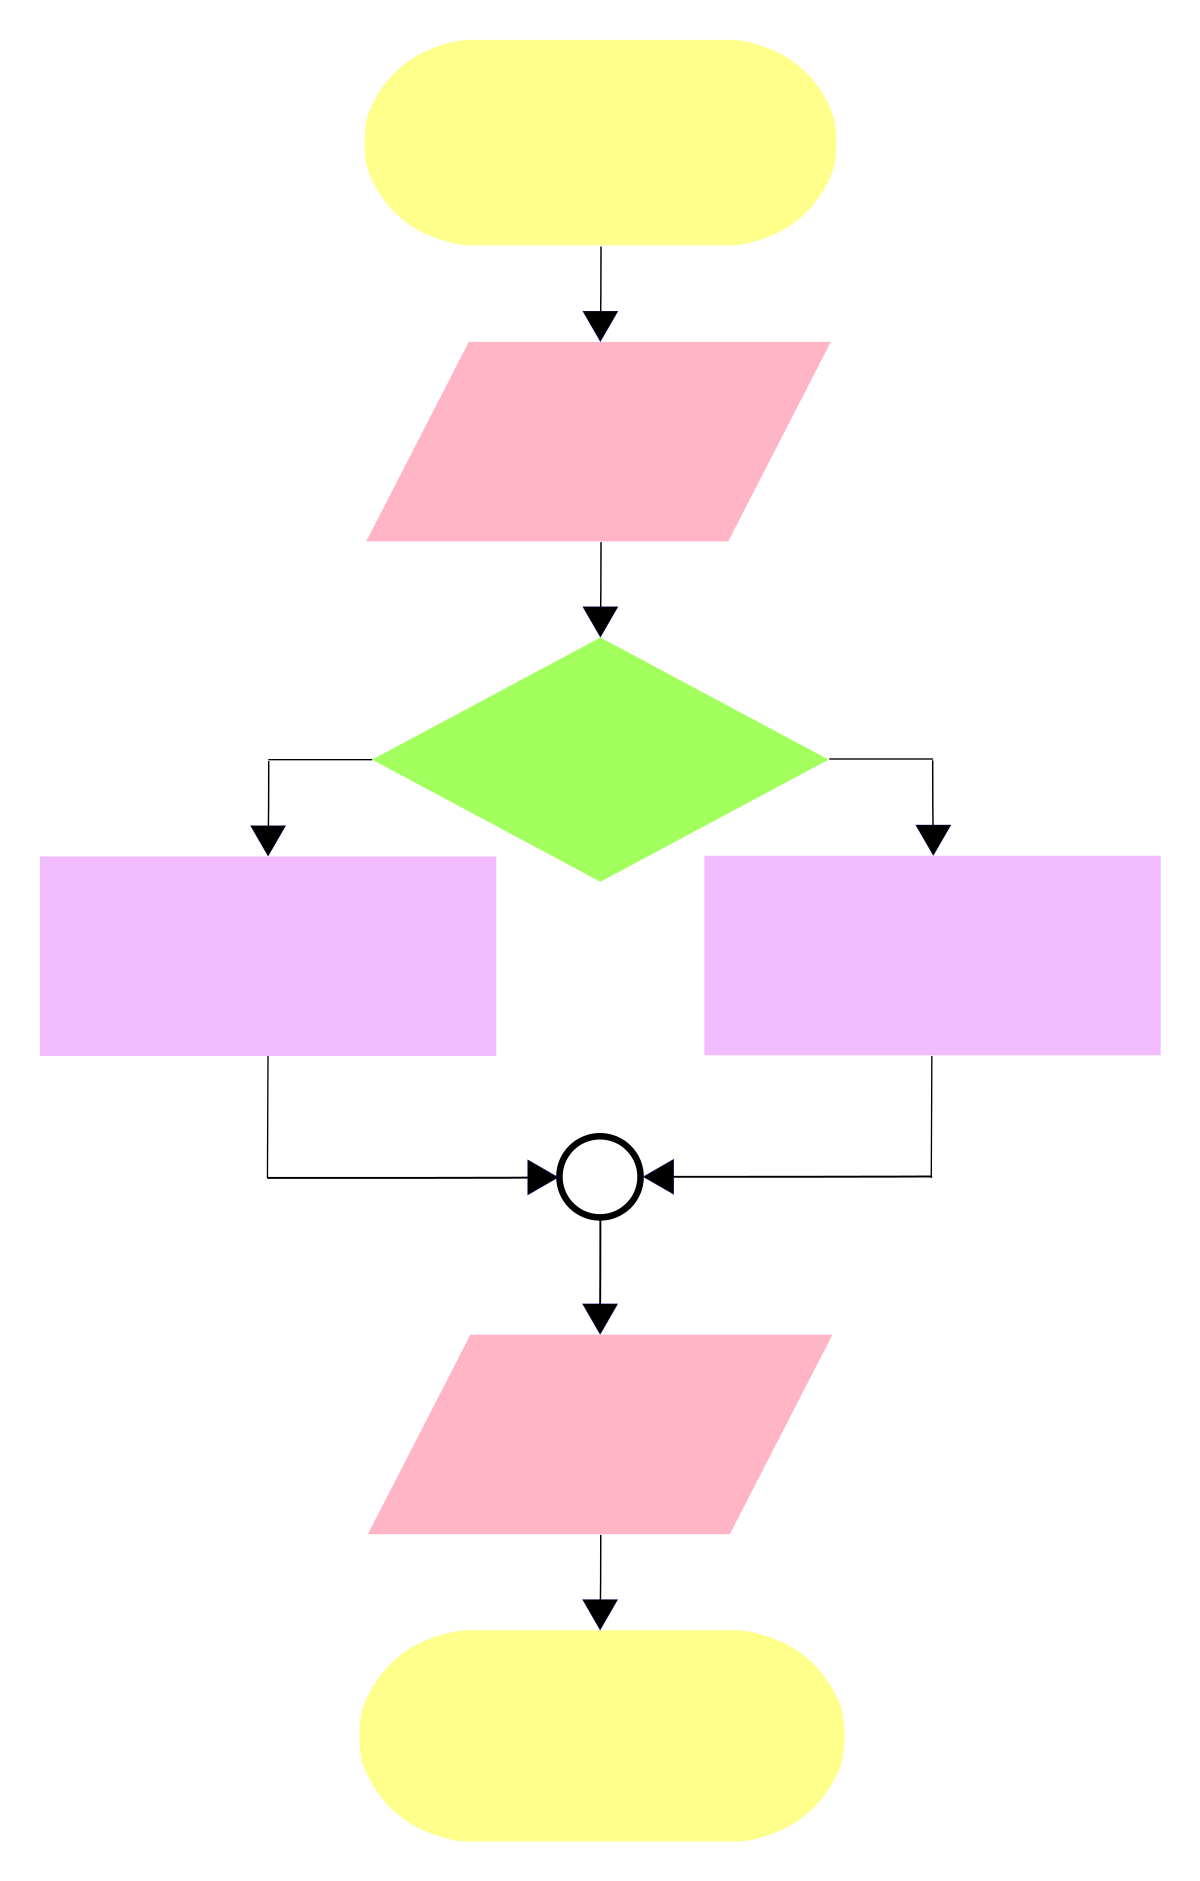
\includegraphics[width=7cm]{./gambar/flowchart.png}
    \caption{Diagram alir penelitian.}
    \label{fig:diagramAlirPenelitian}
\end{figure}


%=====================================================================
\section{Jenis dan Desain Penelitian}
%=====================================================================

...


%=====================================================================
\section{Lokasi dan Waktu Penelitian}
%=====================================================================

...


%=====================================================================
\section{Prosedur Penelitian}
%=====================================================================

%---------------------------------------------------------------------
\subsection{Perangkat Penelitian}
%---------------------------------------------------------------------

%Lorem ipsum.
%\setlist{nolistsep}
%\begin{enumerate}[noitemsep]
%    \item Lorem ipsum.
%    \item ...
%\end{enumerate}


%---------------------------------------------------------------------
\subsection{Langkah Kerja}
%---------------------------------------------------------------------

\vspace{3mm}

\subsubsection{Subsubbagian 1}

%Lorem ipsum.
%\setlist{nolistsep}
%\begin{enumerate}[noitemsep]
%    \item Lorem ipsum.
%    \item ...
%\end{enumerate}

\subsubsection{Subsubbagian 2}

%Lorem ipsum.
%\setlist{nolistsep}
%\begin{enumerate}[noitemsep]
%    \item Lorem ipsum.
%    \item ...
%\end{enumerate}

\subsubsection{Subsubbagian 3}

%Lorem ipsum.
%\setlist{nolistsep}
%\begin{enumerate}[noitemsep]
%    \item Lorem ipsum.
%    \item ...
%\end{enumerate}